\chapter{Conclusiones}

En el final de esta tesis, hay cuatro temas interesantes para analizar.

\vspace{\baselineskip}
El primer tema a analizar es la integración de la exploración a la herramienta MTSA, la cual se puede ver en detalle en el 
siguiente capítulo. 
Se extendió el lenguaje de Procesos de Estados Finitos (FSP) para que sea sencillo definir exploraciones, se agregaron botones 
para dar control total sobre la exploración y se agregó una nueva forma de visualización de los modelos, más flexible, mediante 
la pestaña Layout.

\vspace{\baselineskip}
La herramienta nos permite visualizar la exploración paso a paso, tanto la traza de la exploración como la 
evolución de los modelos. También nos permite avanzar inmediatamente la cantidad de pasos necesarios, para luego ver en detalle 
una etapa más avanzada de la exploración. Es posible explorar siguiendo la estrategia de exploración, e intervenir manualmente 
en las decisiones en caso de ser necesario.

\vspace{\baselineskip}
El segundo tema importante es el algoritmo de exploración. Resuelve el problema correctamente en caso de contar con una estrategia 
adecuada, y tiene la flexibilidad suficiente como para permitir las ventajas mencionadas en el párrafo anterior. Su mayor 
inconveniente es la complejidad temporal.

\vspace{\baselineskip}
Por cada iteración del algoritmo es necesario realizar una síntesis de controladores para decidir si es necesario seguir explorando 
(dos síntesis en el caso de que sea necesario un reset), una síntesis para la estrategia Síntesis, y un número variable de síntesis 
para la estrategia Nueva Acción en caso de que no haya acciones nuevas en el estado actual.

\vspace{\baselineskip}
La síntesis de controladores es un proceso computacionalmente caro. Cada modelo que sintetizamos es muy similar al modelo sintetizado 
en la iteración anterior, sería interesante como trabajo a futuro poder utilizar la síntesis anterior para realizar la próxima en 
vez de volver a realizar el proceso desde el comienzo. Esto afectaría considerablemente el rendimiento del algoritmo en forma favorable.

\vspace{\baselineskip}
El tercer tema interesante surge del ejemplo del laberinto que baja. En los MTSs, al utilizar una transición posible, perdemos la forma 
de especificar que podemos volver exactamente al mismo estado del cual sale la transición posible. Sería de bastante utilidad, como 
trabajo a futuro, extender los MTSs de alguna forma que permita especificar estos detalles.

\begin{figure}[H]
	\centering
		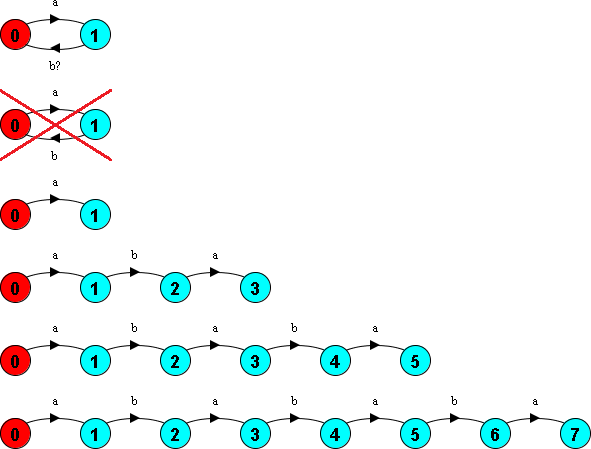
\includegraphics[width=1.0\textwidth]{Imagenes/Otros/Limitaciones.png}
	\caption{Limitaciones del modelado con MTSs}
	\label{fig:Limitaciones}
\end{figure}

Como se puede ver en la imagen, el MTS no se puede refinar al primero de los LTSs, sino que los LTSs que pueden ser refinados a partir 
del MTS son de la forma del segundo LTS en adelante.

\vspace{\baselineskip}
Por último, el cuarto tema fundamental a tener en cuenta es la estrategia presentada. La estrategia resuelve el problema de salir de 
un laberinto, incluso con la participación de agentes externos que influyen sobre el entorno. Pero lo único que busca la estrategia 
es determinar si es posible o no cumplir el objetivo propuesto, como trabajo a futuro se puede mejorar en varios aspectos para reducir 
la cantidad de pasos necesarios para hallar una respuesta.

\vspace{\baselineskip}
Por ejemplo, en caso de tener varias acciones disponibles, siempre las va a elegir basándose en el mismo orden arbitrario. En consecuencia, 
la exploración siempre de preferencia a una dirección por sobre las demás, lo cual puede ser perjudicial. Sería interesante definir 
la forma en la que se elige una acción en caso de que haya varias acciones que cumplen los requisitos de la estrategia, ya sea de forma 
aleatoria o mediante una heurística.

\vspace{\baselineskip}
Algo similar ocurre cuando la estrategia necesita dirigirse hacia otro estado, por encontrarse en un estado completamente explorado. 
En la versión actual de la estrategia se intenta llegar a un estado elegido de forma arbitraria entre los que no fueron completamente 
explorados. Hay varias opciones que podrían llegar a ser más adecuadas, como por ejemplo dirigirse hacia el estado más cercano a la 
posición actual, al más cercano al inicio para hacer una exploración de estilo BFS (Breadth First Search), o al más lejano para explorar 
en forma DFS (Depth First Search) o intentar heurísticas más complicadas, quizás utilizando la información sobre el entorno de la cual 
disponemos en el momento.

\vspace{\baselineskip}
Además de las posibles optimizaciones sobre la estrategia presentada, sería interesante elaborar estrategias nuevas para resolver el 
problema, o estrategias adecuadas para circunstancias particulares, como no disponer de un modelo del entorno, o no poder distinguir 
inequívocamente las posiciones en el entorno.

\vspace{\baselineskip}
En conclusión, este trabajo es un primer paso, el cual brinda las herramientas necesarias para comenzar a investigar el campo de la 
exploración mediante MTSs. Todavía queda mucho por hacer en varios aspectos diferentes, ya que es un tema nuevo, extenso e interesante.